\chapter{Function Hooking and Trampoline-Based Interception}

\section*{Overview}

At the heart of our cheat framework lies a fundamental and widely-used technique: \textbf{function hooking}. This mechanism allows us to intercept and manipulate internal function calls within the game, modify their behavior, and seamlessly resume execution without disrupting the application’s control flow.

\begin{tcolorbox}[colback=gray!10, colframe=gray!10, boxrule=0pt, sharp corners, width=\linewidth, left=1mm, right=1mm, top=0.5mm, bottom=0.5mm]
\textbf{What is Function Hooking?} \\
Function hooking is the practice of redirecting a function’s execution flow to custom code. It enables the interception, modification, or extension of a program’s behavior without access to its source code.
\end{tcolorbox}

Among the various hooking strategies available, the most stable and stealthy is the \textbf{trampoline hook}.  
Trampoline hooking offers a reliable and elegant solution for redirecting code execution to custom payloads while preserving the original function’s logic.

In this chapter, we present an in-depth explanation of trampoline hooks—how they work, why they are effective, and how they can be implemented safely using the \texttt{MinHook} library.

\section{What is a Trampoline Hook?}

A trampoline hook works by overwriting the beginning of a target function with a jump (typically a near relative \texttt{JMP} or an absolute indirect jump) to a custom handler — our hook payload.  
Since this patch modifies the first few bytes of the original function, those instructions must first be preserved to avoid corrupting the original behavior.  
We do this by copying them into a new, executable memory region known as the \textit{trampoline}.

\begin{tcolorbox}[colback=gray!10, colframe=gray!10, boxrule=0pt, sharp corners, width=\linewidth, left=1mm, right=1mm, top=0.5mm, bottom=0.5mm]
\textbf{What is a Trampoline?} \\
A trampoline is a small section of executable memory that stores the original stolen instructions from a hooked function, allowing seamless continuation after custom code executes.
\end{tcolorbox}

Once our custom payload finishes, control passes to the trampoline, which executes the preserved instructions and then jumps back to the original function — resuming normal execution as if nothing had changed.

This redirection process involves four main components:

\begin{itemize}
  \item \textbf{Original (Hooked) Function}: The function entry point is patched to redirect execution.
  \item \textbf{Relay Function}: A lightweight stub that jumps to the hook payload.
  \item \textbf{Hook Payload}: Executes the desired cheat logic before invoking the trampoline.
  \item \textbf{Trampoline}: Holds the stolen instructions and redirects execution back into the original code.
\end{itemize}

\begin{figure}[H]
  \centering
  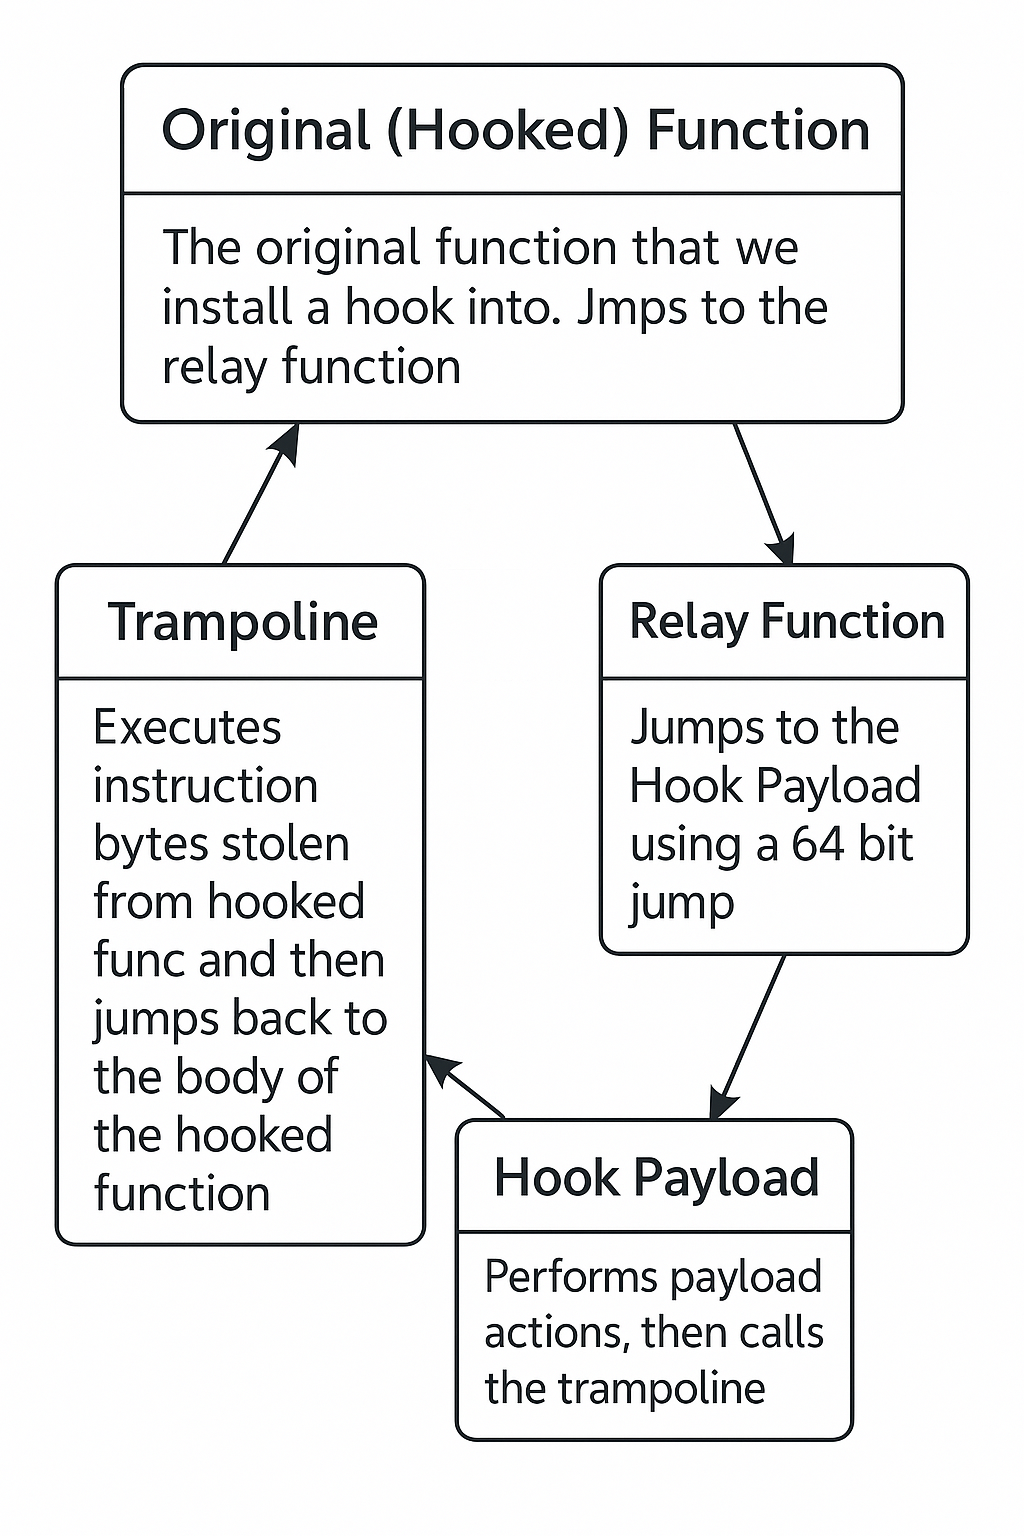
\includegraphics[width=0.55\textwidth]{images/TrampolineFinal.png}
  \caption{Control flow in a trampoline hook setup.}
\end{figure}

\section{Reverse Engineering and Function Discovery}

Before hooking any function, it is essential to identify which ones control the behaviors we want to alter.  
This requires reverse engineering the game’s dynamic libraries—most notably \texttt{client.dll}, which contains the majority of client-side logic.

Using static analysis tools such as \textit{IDA Pro} and \textit{Ghidra}, along with dynamic debugging tools like \textit{x64dbg}, we analyzed exported symbols, disassembled machine code, and traced runtime behavior to locate key functions.


To overcome ASLR, we extracted \textbf{signatures} — short byte sequences unique to each function.  
Our injected DLL scans memory at runtime to locate these signatures and dynamically apply the hooks, ensuring compatibility across different sessions and system restarts.  
The implementation of the pattern scanning logic used for this purpose can be found in our codebase, specifically within the \texttt{helper.cpp} class.

Rather than scanning for static memory addresses—which are often relocated due to ASLR—we focus on scanning for \textbf{instruction bytes}.  
This approach ensures that our patterns remain valid across game updates and memory randomization.  
Typically, patterns include some wildcards (\texttt{??}) to account for dynamic elements such as relative offsets or pointers, which are not fixed between runs.

For instance, one of the patterns we use to locate the view matrix within \texttt{client.dll} is:

\begin{lstlisting}[style=cppstyle]
"48 8D ?? ?? ?? ?? ?? 48 C1 E0 06 48 03 C1 C3 CC CC"
\end{lstlisting}

Here, the \texttt{??} symbols act as \textbf{wildcards}, allowing any byte to match at those positions.  
This flexibility ensures that even if address operands change, the overall pattern remains detectable based on the surrounding instruction sequence.

\section{Why Trampoline Hooks Are Effective}

Trampoline hooks offer several distinct advantages for real-time game manipulation and anti-cheat evasion:

\begin{itemize}
  \item They preserve the game’s original control flow, allowing normal execution to continue after the cheat logic runs.
  \item They maintain stack integrity and valid return addresses, helping to evade detection techniques such as return address validation (used by VAC).
  \item They avoid introducing foreign code into new memory regions, reducing the risk of detection by memory scanners.
\end{itemize}

In short, trampoline hooking provides a balance between flexibility, stability, and stealth — making it the preferred method in both legitimate instrumentation tools and game hacking frameworks.




\section{Implementing Hooks with MinHook}

To install hooks safely, efficiently, and with minimal risk of destabilizing the game, we rely on \textbf{MinHook}—a lightweight, open-source hooking library for x86 and x64 Windows systems.

\begin{tcolorbox}[colback=gray!10, colframe=gray!10, boxrule=0pt, sharp corners, width=\linewidth, left=1mm, right=1mm, top=0.5mm, bottom=0.5mm]
\textbf{What is MinHook?} \\
\textit{MinHook} is a minimalistic and efficient library designed to simplify the process of function hooking. It automatically handles instruction relocation, trampoline creation, and thread-safe patching, offering a robust and reliable solution for both x86 and x64 applications.
\end{tcolorbox}

Our hooking setup follows a clear structure:

\begin{itemize}
    \item A \texttt{typedef} defines the original function’s signature.
    \item A static pointer stores the original (trampoline) function.
    \item A static method implements the custom logic to be executed.
\end{itemize}

First, we define the structure for the hook:

\begin{lstlisting}[style=cppstyle]
// Class responsible for world color modulation hook
class WorldModulation {
public:
    // Typedef for the original function signature
    typedef void* (__fastcall* ModulateWorldColorFn)(...);

    // Pointer to store the original (trampoline) function
    static ModulateWorldColorFn oModulateWorldColor;

    // Our custom hook function
    static void* __fastcall hModulateWorldColor(...);
};

// Instance of the class
WorldModulation m_WorldModulation;
\end{lstlisting}

Installing the hook with \textbf{MinHook} is straightforward:

\begin{lstlisting}[style=cppstyle]
// Function to initialize and install the hook
void InitHook() {
    MH_Initialize(); // Initialize MinHook library

    // Create a hook: redirect TargetAddress to our custom function
    MH_CreateHook((LPVOID)TargetAddress, &WorldModulation::hModulateWorldColor, (LPVOID*)&WorldModulation::oModulateWorldColor);

    MH_EnableHook((LPVOID)TargetAddress); // Enable the installed hook
}
\end{lstlisting}

The custom hook function applies a global color modulation if necessary:

\begin{lstlisting}[style=cppstyle]
// Custom function that replaces the original behavior
void* __fastcall WorldModulation::hModulateWorldColor(...) {
    // Check if world modulation is enabled
    if (!Globals::worldModulation)
        return oModulateWorldColor(...); // If not, just call the original function

    // Apply the global color to all world objects
    for (int i = 0; i < pWorld->count; i++) {
        auto& obj = pWorld->array[i];
        obj.SetColor(Globals::worldModulationColor); // Apply the new color
    }

    // After custom logic, continue execution normally
    return oModulateWorldColor(...);
}
\end{lstlisting}

This structure ensures that our custom logic only executes when necessary, preserving the original behavior otherwise.

\section{Final Thoughts on Trampoline Hooking}

\textbf{Trampoline hooking} provides a \textit{stable}, \textit{stealthy}, and \textit{flexible} method for manipulating in-game behavior while minimizing the risk of detection or instability.

By carefully preserving \textbf{return addresses}, maintaining \textbf{control flow integrity}, and avoiding the introduction of foreign memory regions, trampoline hooks form the \textbf{foundation} of an effective and resilient cheat architecture.

The typical workflow begins with \textbf{reverse engineering} target DLLs to identify relevant functions, \textbf{generating dynamic signatures} for reliable location at runtime, and \textbf{installing hooks} using safe, battle-tested libraries like \textbf{MinHook}.  
This method ensures that our modifications remain compatible even as the game's memory layout evolves between sessions or updates.

In the next chapter, we will explore \textbf{advanced techniques} for identifying and prioritizing the most impactful functions to hook, particularly those related to \textit{rendering}, \textit{game logic processing}, and \textit{player state management}.
